


% HOT TOPICS:
%  - Figures
%  - ECA Paradigm explanation
%  - 





\documentclass[11pt]{article}%,twocolumn
\usepackage{url}
\usepackage{cite}
\usepackage{graphicx}
\usepackage{listings}
\usepackage{colortbl}
\usepackage{fancyvrb}
\usepackage{color}
\usepackage[ascii]{inputenc}
\usepackage{titling}
\usepackage{titlesec}
\usepackage[toc,page]{appendix}
%\usepackage[titletoc]{appendix}
\newcommand{\subtitle}[1]{%
  \posttitle{%
    \par\end{center}
    \begin{center}\large#1\end{center}
    \vskip0.5em}%
}
\setlength{\parskip}{\baselineskip}
\titlespacing\section{0pt}{12pt plus 4pt minus 2pt}{0pt plus 2pt minus 2pt}
\titlespacing\subsection{0pt}{10pt plus 3pt minus 1pt}{0pt plus 1pt minus 1pt}
\titlespacing\subsubsection{0pt}{8pt plus 2pt minus 0pt}{0pt plus 0pt minus 0pt}


\makeatletter
\def\PY@reset{\let\PY@it=\relax \let\PY@bf=\relax%
    \let\PY@ul=\relax \let\PY@tc=\relax%
    \let\PY@bc=\relax \let\PY@ff=\relax}
\def\PY@tok#1{\csname PY@tok@#1\endcsname}
\def\PY@toks#1+{\ifx\relax#1\empty\else%
    \PY@tok{#1}\expandafter\PY@toks\fi}
\def\PY@do#1{\PY@bc{\PY@tc{\PY@ul{%
    \PY@it{\PY@bf{\PY@ff{#1}}}}}}}
\def\PY#1#2{\PY@reset\PY@toks#1+\relax+\PY@do{#2}}

\expandafter\def\csname PY@tok@gd\endcsname{\def\PY@tc##1{\textcolor[rgb]{0.63,0.00,0.00}{##1}}}
\expandafter\def\csname PY@tok@gu\endcsname{\let\PY@bf=\textbf\def\PY@tc##1{\textcolor[rgb]{0.50,0.00,0.50}{##1}}}
\expandafter\def\csname PY@tok@gt\endcsname{\def\PY@tc##1{\textcolor[rgb]{0.00,0.27,0.87}{##1}}}
\expandafter\def\csname PY@tok@gs\endcsname{\let\PY@bf=\textbf}
\expandafter\def\csname PY@tok@gr\endcsname{\def\PY@tc##1{\textcolor[rgb]{1.00,0.00,0.00}{##1}}}
\expandafter\def\csname PY@tok@cm\endcsname{\let\PY@it=\textit\def\PY@tc##1{\textcolor[rgb]{0.25,0.50,0.50}{##1}}}
\expandafter\def\csname PY@tok@vg\endcsname{\def\PY@tc##1{\textcolor[rgb]{0.10,0.09,0.49}{##1}}}
\expandafter\def\csname PY@tok@m\endcsname{\def\PY@tc##1{\textcolor[rgb]{0.40,0.40,0.40}{##1}}}
\expandafter\def\csname PY@tok@mh\endcsname{\def\PY@tc##1{\textcolor[rgb]{0.40,0.40,0.40}{##1}}}
\expandafter\def\csname PY@tok@go\endcsname{\def\PY@tc##1{\textcolor[rgb]{0.53,0.53,0.53}{##1}}}
\expandafter\def\csname PY@tok@ge\endcsname{\let\PY@it=\textit}
\expandafter\def\csname PY@tok@vc\endcsname{\def\PY@tc##1{\textcolor[rgb]{0.10,0.09,0.49}{##1}}}
\expandafter\def\csname PY@tok@il\endcsname{\def\PY@tc##1{\textcolor[rgb]{0.40,0.40,0.40}{##1}}}
\expandafter\def\csname PY@tok@cs\endcsname{\let\PY@it=\textit\def\PY@tc##1{\textcolor[rgb]{0.25,0.50,0.50}{##1}}}
\expandafter\def\csname PY@tok@cp\endcsname{\def\PY@tc##1{\textcolor[rgb]{0.74,0.48,0.00}{##1}}}
\expandafter\def\csname PY@tok@gi\endcsname{\def\PY@tc##1{\textcolor[rgb]{0.00,0.63,0.00}{##1}}}
\expandafter\def\csname PY@tok@gh\endcsname{\let\PY@bf=\textbf\def\PY@tc##1{\textcolor[rgb]{0.00,0.00,0.50}{##1}}}
\expandafter\def\csname PY@tok@ni\endcsname{\let\PY@bf=\textbf\def\PY@tc##1{\textcolor[rgb]{0.60,0.60,0.60}{##1}}}
\expandafter\def\csname PY@tok@nl\endcsname{\def\PY@tc##1{\textcolor[rgb]{0.63,0.63,0.00}{##1}}}
\expandafter\def\csname PY@tok@nn\endcsname{\let\PY@bf=\textbf\def\PY@tc##1{\textcolor[rgb]{0.00,0.00,1.00}{##1}}}
\expandafter\def\csname PY@tok@no\endcsname{\def\PY@tc##1{\textcolor[rgb]{0.53,0.00,0.00}{##1}}}
\expandafter\def\csname PY@tok@na\endcsname{\def\PY@tc##1{\textcolor[rgb]{0.49,0.56,0.16}{##1}}}
\expandafter\def\csname PY@tok@nb\endcsname{\def\PY@tc##1{\textcolor[rgb]{0.00,0.50,0.00}{##1}}}
\expandafter\def\csname PY@tok@nc\endcsname{\let\PY@bf=\textbf\def\PY@tc##1{\textcolor[rgb]{0.00,0.00,1.00}{##1}}}
\expandafter\def\csname PY@tok@nd\endcsname{\def\PY@tc##1{\textcolor[rgb]{0.67,0.13,1.00}{##1}}}
\expandafter\def\csname PY@tok@ne\endcsname{\let\PY@bf=\textbf\def\PY@tc##1{\textcolor[rgb]{0.82,0.25,0.23}{##1}}}
\expandafter\def\csname PY@tok@nf\endcsname{\def\PY@tc##1{\textcolor[rgb]{0.00,0.00,1.00}{##1}}}
\expandafter\def\csname PY@tok@si\endcsname{\let\PY@bf=\textbf\def\PY@tc##1{\textcolor[rgb]{0.73,0.40,0.53}{##1}}}
\expandafter\def\csname PY@tok@s2\endcsname{\def\PY@tc##1{\textcolor[rgb]{0.73,0.13,0.13}{##1}}}
\expandafter\def\csname PY@tok@vi\endcsname{\def\PY@tc##1{\textcolor[rgb]{0.10,0.09,0.49}{##1}}}
\expandafter\def\csname PY@tok@nt\endcsname{\let\PY@bf=\textbf\def\PY@tc##1{\textcolor[rgb]{0.00,0.50,0.00}{##1}}}
\expandafter\def\csname PY@tok@nv\endcsname{\def\PY@tc##1{\textcolor[rgb]{0.10,0.09,0.49}{##1}}}
\expandafter\def\csname PY@tok@s1\endcsname{\def\PY@tc##1{\textcolor[rgb]{0.73,0.13,0.13}{##1}}}
\expandafter\def\csname PY@tok@sh\endcsname{\def\PY@tc##1{\textcolor[rgb]{0.73,0.13,0.13}{##1}}}
\expandafter\def\csname PY@tok@sc\endcsname{\def\PY@tc##1{\textcolor[rgb]{0.73,0.13,0.13}{##1}}}
\expandafter\def\csname PY@tok@sx\endcsname{\def\PY@tc##1{\textcolor[rgb]{0.00,0.50,0.00}{##1}}}
\expandafter\def\csname PY@tok@bp\endcsname{\def\PY@tc##1{\textcolor[rgb]{0.00,0.50,0.00}{##1}}}
\expandafter\def\csname PY@tok@c1\endcsname{\let\PY@it=\textit\def\PY@tc##1{\textcolor[rgb]{0.25,0.50,0.50}{##1}}}
\expandafter\def\csname PY@tok@kc\endcsname{\let\PY@bf=\textbf\def\PY@tc##1{\textcolor[rgb]{0.00,0.50,0.00}{##1}}}
\expandafter\def\csname PY@tok@c\endcsname{\let\PY@it=\textit\def\PY@tc##1{\textcolor[rgb]{0.25,0.50,0.50}{##1}}}
\expandafter\def\csname PY@tok@mf\endcsname{\def\PY@tc##1{\textcolor[rgb]{0.40,0.40,0.40}{##1}}}
%\expandafter\def\csname PY@tok@err\endcsname{\def\PY@bc##1{\setlength{\fboxsep}{0pt}\fcolorbox[rgb]{1.00,0.00,0.00}{1,1,1}{\strut ##1}}}
\expandafter\def\csname PY@tok@kd\endcsname{\let\PY@bf=\textbf\def\PY@tc##1{\textcolor[rgb]{0.00,0.50,0.00}{##1}}}
\expandafter\def\csname PY@tok@ss\endcsname{\def\PY@tc##1{\textcolor[rgb]{0.10,0.09,0.49}{##1}}}
\expandafter\def\csname PY@tok@sr\endcsname{\def\PY@tc##1{\textcolor[rgb]{0.73,0.40,0.53}{##1}}}
\expandafter\def\csname PY@tok@mo\endcsname{\def\PY@tc##1{\textcolor[rgb]{0.40,0.40,0.40}{##1}}}
\expandafter\def\csname PY@tok@kn\endcsname{\let\PY@bf=\textbf\def\PY@tc##1{\textcolor[rgb]{0.00,0.50,0.00}{##1}}}
\expandafter\def\csname PY@tok@mi\endcsname{\def\PY@tc##1{\textcolor[rgb]{0.40,0.40,0.40}{##1}}}
\expandafter\def\csname PY@tok@gp\endcsname{\let\PY@bf=\textbf\def\PY@tc##1{\textcolor[rgb]{0.00,0.00,0.50}{##1}}}
\expandafter\def\csname PY@tok@o\endcsname{\def\PY@tc##1{\textcolor[rgb]{0.40,0.40,0.40}{##1}}}
\expandafter\def\csname PY@tok@kr\endcsname{\let\PY@bf=\textbf\def\PY@tc##1{\textcolor[rgb]{0.00,0.50,0.00}{##1}}}
\expandafter\def\csname PY@tok@s\endcsname{\def\PY@tc##1{\textcolor[rgb]{0.73,0.13,0.13}{##1}}}
\expandafter\def\csname PY@tok@kp\endcsname{\def\PY@tc##1{\textcolor[rgb]{0.00,0.50,0.00}{##1}}}
\expandafter\def\csname PY@tok@w\endcsname{\def\PY@tc##1{\textcolor[rgb]{0.73,0.73,0.73}{##1}}}
\expandafter\def\csname PY@tok@kt\endcsname{\def\PY@tc##1{\textcolor[rgb]{0.69,0.00,0.25}{##1}}}
\expandafter\def\csname PY@tok@ow\endcsname{\let\PY@bf=\textbf\def\PY@tc##1{\textcolor[rgb]{0.67,0.13,1.00}{##1}}}
\expandafter\def\csname PY@tok@sb\endcsname{\def\PY@tc##1{\textcolor[rgb]{0.73,0.13,0.13}{##1}}}
\expandafter\def\csname PY@tok@k\endcsname{\let\PY@bf=\textbf\def\PY@tc##1{\textcolor[rgb]{0.00,0.50,0.00}{##1}}}
\expandafter\def\csname PY@tok@se\endcsname{\let\PY@bf=\textbf\def\PY@tc##1{\textcolor[rgb]{0.73,0.40,0.13}{##1}}}
\expandafter\def\csname PY@tok@sd\endcsname{\let\PY@it=\textit\def\PY@tc##1{\textcolor[rgb]{0.73,0.13,0.13}{##1}}}
%\expandafter\def\csname PY@tok@err\endcsname{}

\def\PYZbs{\char`\\}
\def\PYZus{\char`\_}
\def\PYZob{\char`\{}
\def\PYZcb{\char`\}}
\def\PYZca{\char`\^}
\def\PYZam{\char`\&}
\def\PYZlt{\char`\<}
\def\PYZgt{\char`\>}
\def\PYZsh{\char`\#}
\def\PYZpc{\char`\%}
\def\PYZdl{\char`\$}
\def\PYZhy{\char`\-}
\def\PYZsq{\char`\'}
\def\PYZdq{\char`\"}
\def\PYZti{\char`\~}
% for compatibility with earlier versions
\def\PYZat{@}
\def\PYZlb{[}
\def\PYZrb{]}
\makeatother

%\pretitle{\begin{center}Master Thesis Report\\\vspace*{4 mm}\today\end{center}\vspace*{15 mm}\begin{center}}

%\posttitle{\end{center}\begin{center}\end{center}}

\begin{document}

\title{\huge Towards The Reactive Web\vspace*{15 mm}}
%\subtitle{Master Thesis Report}
\date{\today}
%\date{}
%\author{Dominic Bosch \\ Departement Mathematics and Computer Science \\ University of Basel}
\author{\fontsize{11}{9}\selectfont
Master Thesis\\
\vspace*{10 mm}\\
Dominic Bosch\\
Departement Mathematics and Computer Science\\
University of Basel
}
\maketitle

\renewcommand{\abstractname}{}
\begin{abstract}
\textbf{Abstract.}

T.B.D.

\end{abstract}


\newpage
\tableofcontents
\newpage



\section{Introduction}
% NOTES / TODOs:
%
% Take from preparation
%
% Definitions! need to be in text
% WebAPI
% Engine
% Event Poller
% Action Invoker
% Rules
% Rule Language (JSON Object?)
% Reactivity
% Programmablity of the web


% SYSTEM??? what do we call it in the theory part?
% what do we call it when we talk about the prototype system??
% Do I reference my own work?


The fast evolving web has brought up a trend towards easy to master interfaces to services, the so called WebAPIs.
They do not only provide access to mere services but whole applications that allow access over WebAPIs.
These trending WebAPIs benefit from a RESTful architecture which predominantly uses HTTP and thus relies on the most basic and powerful operations and the basis of the Web itself, the HTTP protocol. 

quick (handling/mastering) accessible services and even whole web applications through so called Web APIs.
WebAPIs provide powerful tools to govern data and functionality in the web independently of any user interface from the service provider.
The relatively
Allowing access to these services via API is increasingly popular and allows to mash up these services

Practically all services flood the user with events
The web should be event driven, that's why we need an engine that deals with events and makes the web reactive
There's still the challenge of filtering
What's important to whom
Plus the user needs to have tools to combine and add programmability to the combination,( such as conditions, selection of provided arguments and so on)



\subsection{Related Work}
% NOTES / TODOs:
%
% Zapier, IFTTT
% import.io
% Show kynetix?

% Grunt to build project
% jsprime to make code safe
% stylus for css
% (Categorized section at the end about existing rule languages)

\subsubsection{WebAPI Mashups}
Mashups combine information and functionality of more than one resource in a single place.
The mashing up of such resources allows new points of view on data, or even ways to interact with them.
Simple functions are combined into more powerful ones which influence data and services in a way their founders eventually didn't even think of.
They have been developped ever since services in the web started to exist and were accessible in a more or less convenient way.
One of the earliest inventors of such a webservice mashup is Paul Rademacher.
In the same year after Google Maps came up in 2005, he invented a site\cite{wwwRademacherOne,wwwRademacherTwo} that displayed Craigslist houses on a Google Map.
With no Google Maps API at that time, he needed time and skills to reverse engineer Google Map's functionalities.


A large number of such "static" mashups were and are still developped.
They are static in the way that they aggregate a fixed (and mostly low) number, of either data or functionality resources, to provide an enhanced resource in a specialized domain.
Of course Mashups can be mashed up again, to provide even more sophisticated functionality and data.
Some latest example Mashups, taken from the ProgrammableWeb\cite{wwwProgrammableWeb} directory, are:

\begin{itemize}
  \item Wifi and Plugs\cite{wwwWifiAndPlugs}: MapBox, Google Docs and Import.io API's used to display where Wi-Fi and plugs are available in London.
  \item MapLight\cite{wwwMapLight}: GovTrack.us and OpenSecrets API's used to combine political results with financial contributions to show how capital contributions affect voting.
  \item Shared Count\cite{wwwSharedCount}: Facebook, LinkedIn, Pinterest and Twitter API's used to display informations about how well spread a URL is on social media sites.
\end{itemize}

In the past few years, research and development for platforms to allow users to flexibly mashup WebAPIs got attention.
With IFTTT and Zapier, two platforms have evolved out of this process.
Users that register on those platforms are provided with a multitude of WebAPI functions that act as event triggers and such that are used to execute actions.
The user is then free to combine these event triggers and actions in the way it suits best, creating helpful WebAPI mashups on their own.

% Since this is a quite new field the why and how is hidden from the research.
% you need events
% you need rules / rule language


\section{Conceptual Model for Reactive Web Systems}
% NOTES / TODOs:
%
% Rahmenbedingungen
% Vorzuege
% Notwendigkeiten
% Architektur


\subsection{Event Condition Action (ECA) Model in the Web}
% NOTES / TODOs:
%
% Model / Schema
% Zeit / Verteiltheit
% RL <-> ECA
% why are we now suddenly responsive? we loosened up certain things

Existing ECA systems (List examples) all act on local data.
Looking at (Wikipedia...) their definition is actions on local data.
This does only add reactivity to these systems and not to the Web per se.

Such systems are merely event sinks which add fairly any value to the Web, except for the individual users and the system itself.
We are taking a step further and allow not only the chaining up of several remote ECA engines, but also the invocation of actions on any arbitrary Web accessible service.



\section{The "XYZ" Prototype System}
% NOTES / TODOs:
%
% Architecture scheme, implementation
% callback functions, hot plugin
% js-select selectors
% List of condition operators
% Why JS, why wasnt it used before? is it used now?
% Transactions in businesses, find use case. how would we lose events?
% Terminierungsproblem (compiler bau), loesungsansaetze



\subsection{Gathering Event Triggers}

Event Gathering is the E in ECA and without one of these letters such a system would not run.
It is of utmost importance to find as much as possible ways to get data into a system.



\subsubsection{Polling for Events}



\subsubsection{Webhooks}
Which 



\subsection{Actions}



\subsection{ECA Rules}



\subsection{Architecture}



\subsection{Complexity in Asynchronous Systems}
% NOTES / TODOs:
%
% Variable bindings
% Asynchronity and Closures
% Closures (https://developer.mozilla.org/en-US/docs/Web/JavaScript/Guide/Closures)$
% Closures are functions that refer to independent (free) variables. 
% In other words, the function defined in the closure 'remembers' the environment in which it was created in. 

% Error tracing

% Apply variable number of function arguments to function



\section{Discussion \& Results}



\subsection{Use Cases}
% NOTES / TODOs:
%
% Temperature warning, using import.io
% Tutorial example: as seen by user, as seen by the developer
%http://khanlou.com/2014/03/model-view-whatever/

\newpage


\section{Future Work}
% NOTES / TODOs:
%
% CEP
We have seen that the ECA approach is already a powerful one to make the web reactive.
A future improvement of this could be to adopt Complex Event Processing (CEP).
This would mean that several events could be stored in a rule and be evaluated in terms of time constraints.
Through this more complex events can be created as a result of several atomic events which would lead into semantically more complex events.
A change in paradigm will result in an approach where events are not just processed when they are entering the system and evaluated against rules, but these events would need to be stored for quite a long time.
Also the rules will not all be checked for each event but they are subject to a scheduler.
It can be decided when and how often a rule is evaluated and all events will be checked at these point in times, whether they are candidates for firing the rule.
A relational database will be needed in order to search through the timestamps


\bibliography{thesisbib}
\bibliographystyle{thesisbst}

\newpage
\renewcommand*\appendixpagename{APPENDIX}
\renewcommand*\appendixtocname{APPENDIX}
%\begin{appendices}
 % \section{ECA Rules Engine Resources}
  %  \subsection{Node.js Rules Engine Code}
   % \subsubsection{ecaserver.js}

    \begin{Verbatim}[fontsize=\small,commandchars=\\\{\}]
    \PY{l+s}{\PYZsq{}}\PY{l+s}{use strict}\PY{l+s}{\PYZsq{}}\PY{p}{;}
    \PY{n}{var} \PY{n}{express} \PY{o}{=} \PY{n}{require}\PY{p}{(}\PY{l+s}{\PYZsq{}}\PY{l+s}{express}\PY{l+s}{\PYZsq{}}\PY{p}{)}\PY{p}{;}
    \PY{n}{var} \PY{n}{qs} \PY{o}{=} \PY{n}{require}\PY{p}{(}\PY{l+s}{\PYZsq{}}\PY{l+s}{querystring}\PY{l+s}{\PYZsq{}}\PY{p}{)}\PY{p}{;}
    \PY{n}{var} \PY{n}{engine} \PY{o}{=} \PY{n}{require}\PY{p}{(}\PY{l+s}{\PYZsq{}}\PY{l+s}{./ecainference}\PY{l+s}{\PYZsq{}}\PY{p}{)}\PY{p}{;}
    \end{Verbatim}
%t.b.d.
%\end{appendices}

\newpage
% WECAST

% WebAPI
% ECA
% Engine
% Reactive
% Web
% Demo
% WebAPI
% System
% Services
% Multipurpose 
% Prototype
% Kernel
% General-Purpose
% Programmable

% Programmable Web 
% General-Purpose ECA Engine Kernel


\textbf{Examples for XYZ:}
\begin{itemize}
  \item \textbf{GEEK} (General-Purpose ECA Engine Kernel)
  \item \textbf{DECADE} (Dynamic ECA Demo Engine)
  \item \textbf{WECAST} (WebAPI ECA Service Trigger)
  \item \textbf{RECAST} (Reactive ECA Service Trigger)
  \item \textbf{PECAN} (Productive ECA eNgine)
  \item \textbf{ICECAP} (Inet-Service Calls through ECA Paradigm)
\end{itemize}




\newpage
\begin{figure*}[htb]
%\begin{center}
\centering
%,angle=-90
  \makebox[\textwidth][c]{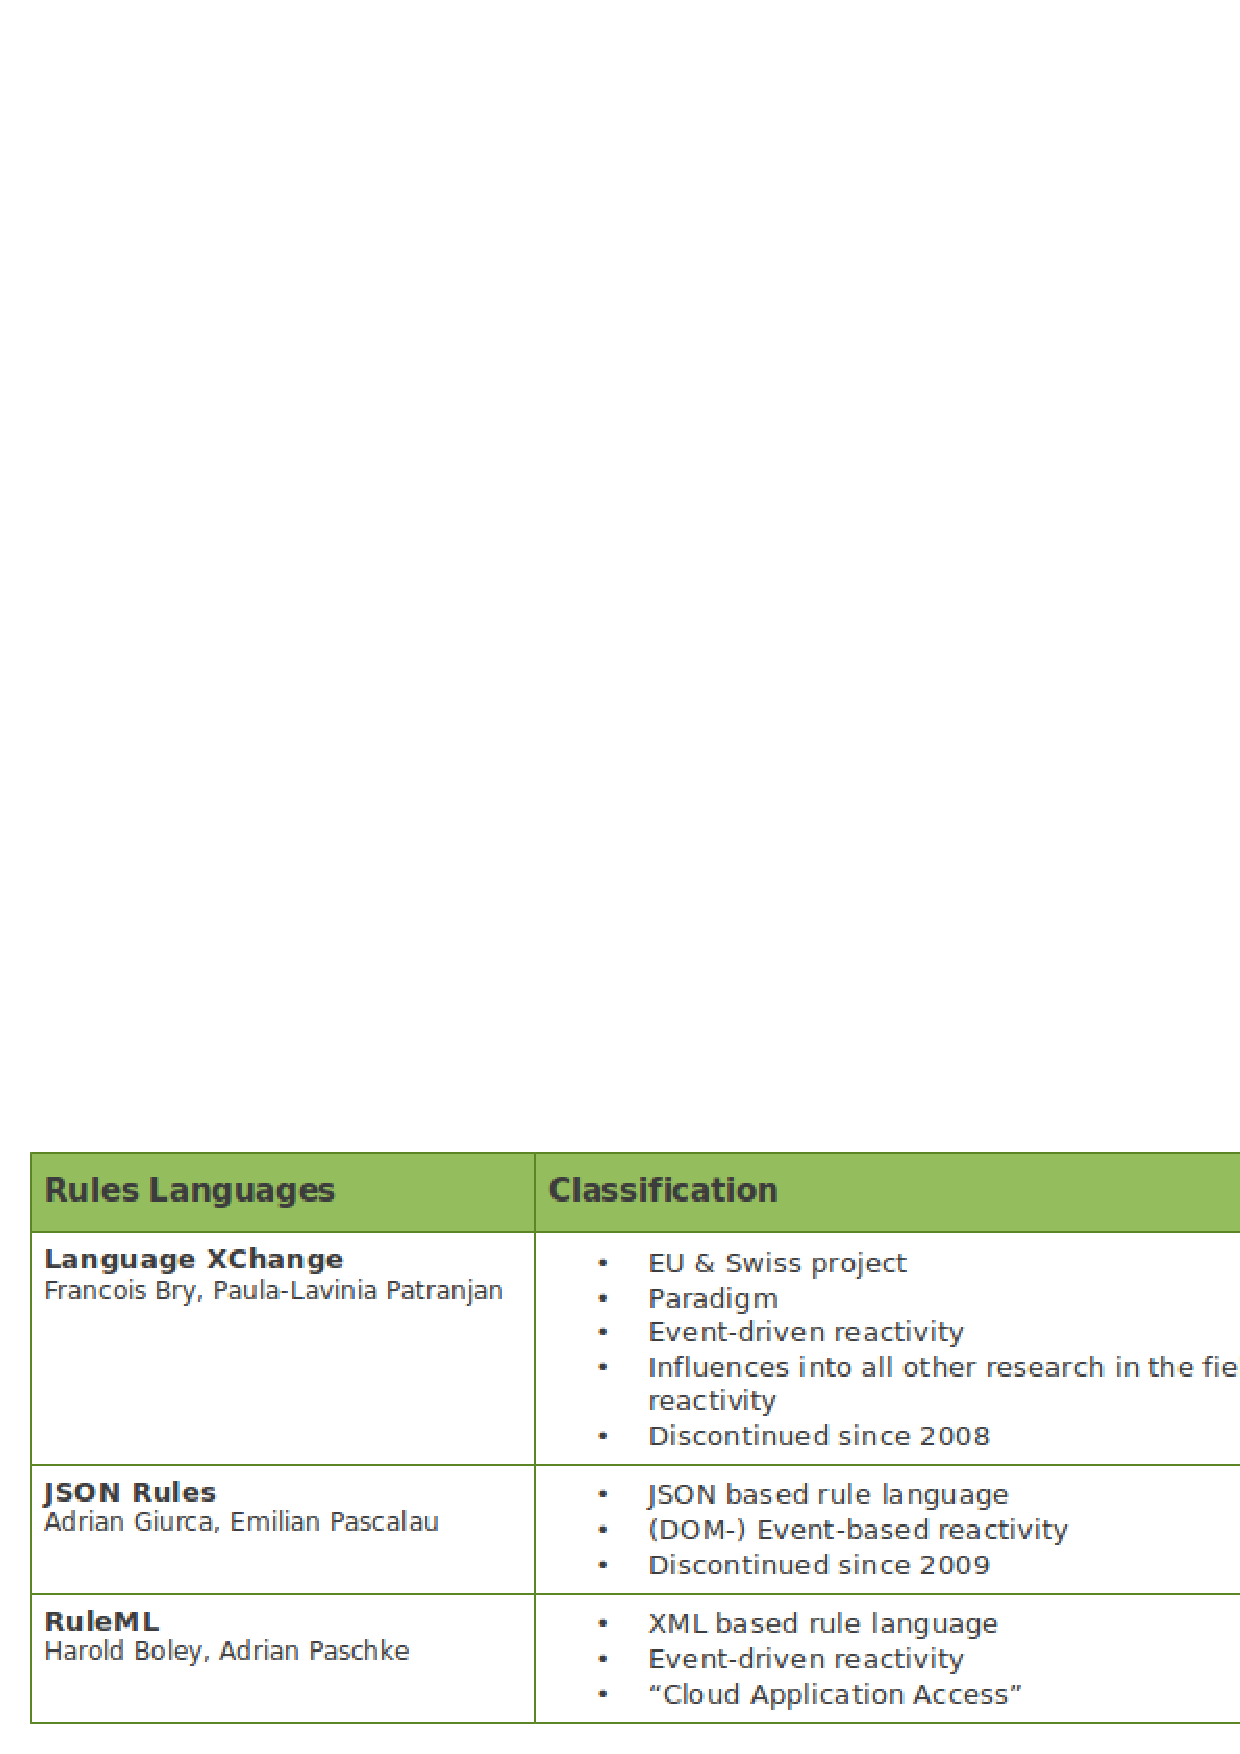
\includegraphics[scale=0.6]{img_rw_1_large}}%
\caption{Examined Rules Languages}
%\end{center}
\end{figure*}

%\section{Related Work}

%\subsection{Rules Languages}
\cite{2009-Paschke_Boley-RCER.pdf} gave a good oveview over existing approaches in 2009.
In this section we examine different existing rule languages with respect to a simple use case.
We want the rule language react on the receipt of an email (event), check for a distinct email address (condition) and store it in a remote location, via a Web API (action).
The email only contains the parts we require for this use case (the sender and a subject). A JSON representation of the email would be:
\begin{Verbatim}[fontsize=\small,commandchars=\\\{\}]
\PY{p}{\PYZob{}}
  \PY{l+s}{\PYZdq{}}\PY{l+s}{event}\PY{l+s}{\PYZdq{}}\PY{p}{:} \PY{l+s}{\PYZdq{}}\PY{l+s}{email}\PY{l+s}{\PYZdq{}}\PY{p}{,}
  \PY{l+s}{\PYZdq{}}\PY{l+s}{sender}\PY{l+s}{\PYZdq{}}\PY{p}{:} \PY{l+s}{\PYZdq{}}\PY{l+s}{sender@mail.com}\PY{l+s}{\PYZdq{}}\PY{p}{,}
  \PY{l+s}{\PYZdq{}}\PY{l+s}{subject}\PY{l+s}{\PYZdq{}}\PY{p}{:} \PY{l+s}{\PYZdq{}}\PY{l+s}{An important message!}\PY{l+s}{\PYZdq{}}
\PY{p}{\PYZcb{}}
\end{Verbatim}


\newpage
%\subsubsection{RDF \& XML}
An early ECA Rule Language for XML repositories\cite{Papamarkos03event-condition-actionrule} was postulated in 2003 and was picked up by many researches afterwards. It was designed to react on insert and delete events within XML repositories and as an action change XML documents.

\begin{Verbatim}[fontsize=\small,commandchars=\\\{\}]
\PY{n}{ON} \PY{n}{INSERT} \PY{n}{document}\PY{p}{(}\PY{l+s}{\PYZsq{}}\PY{l+s}{inbound\PYZus{}queue.xml}\PY{l+s}{\PYZsq{}}\PY{p}{)}\PY{o}{/}\PY{n}{mails}\PY{o}{/}\PY{n}{mail}
\PY{n}{IF} \PY{err}{\PYZdl{}}\PY{n}{delta}\PY{o}{/}\PY{n}{sender}\PY{p}{[}\PY{o}{.}\PY{o}{=}\PY{l+s}{\PYZsq{}}\PY{l+s}{sender@mail.com}\PY{l+s}{\PYZsq{}}\PY{p}{]}
\PY{n}{DO} \PY{n}{DELETE} \PY{n}{document}\PY{p}{(}\PY{l+s}{\PYZsq{}}\PY{l+s}{inbound\PYZus{}queue.xml}\PY{l+s}{\PYZsq{}}\PY{p}{)}\PY{o}{/}\PY{n}{mails}\PY{o}{/}\PY{n}{mail}\PY{p}{;}
   \PY{n}{LET} \PY{err}{\PYZdl{}}\PY{n}{api} \PY{o}{=} \PY{n}{resource}\PY{p}{(}\PY{l+s}{\PYZdq{}}\PY{l+s}{www.webapi.com}\PY{l+s}{\PYZdq{}}\PY{p}{)} \PY{n}{IN}
   \PY{n}{INSERT} \PY{p}{(}\PY{err}{\PYZdl{}}\PY{n}{api}\PY{p}{,} \PY{n}{newcontent}\PY{p}{,} 
      \PY{o}{\PYZlt{}}\PY{n}{content}\PY{o}{\PYZgt{}}\PY{n}{New} \PY{n}{mail}\PY{p}{:} \PY{p}{\PYZob{}}\PY{err}{\PYZdl{}}\PY{n}{delta}\PY{o}{/}\PY{n}{subject}\PY{p}{\PYZcb{}}\PY{o}{\PYZlt{}}\PY{o}{/}\PY{n}{content}\PY{o}{\PYZgt{}}\PY{p}{)}
\end{Verbatim}

Now apart from implementing a rules engine, we would also need to add an XML document event manager which interpretes and pushes events into the XML file \emph{inbound\_queue.xml}. Then again this instance would interprete the ouptuts of the ECA engine, which would theoretically manifest in other XML documents, and produce meaningful actions on remote hosts. This wouldn't be an architecture which has its focus on the solution of our use case and, as a result, add complexity and create an unnecessary overhead.

%\subsubsection{Notation 3}
To make the lengthy RDF definitions smaller and more readable, Notation 3\cite{wwwn3} was designed and announced in 2005. Through the implies operator(=\textgreater) an "event" can be connected to an "action", both expressed in RDF's subject, predicate, object notation, which makes the expression of ECA rules a complicated and not very intuitive task. A solution to our use case would look as follows:

\begin{Verbatim}[fontsize=\small,commandchars=\\\{\}]
\PY{p}{\PYZob{}} \PY{err}{?}\PY{n}{x} \PY{p}{:}\PY{n}{event} \PY{l+s}{\PYZdq{}}\PY{l+s}{email}\PY{l+s}{\PYZdq{}}\PY{o}{.} \PY{err}{?}\PY{n}{x} \PY{p}{:}\PY{n}{sender} \PY{l+s}{\PYZdq{}}\PY{l+s}{sender@mail.com}\PY{l+s}{\PYZdq{}} \PY{p}{\PYZcb{}} 
    \PY{o}{=}\PY{o}{\PYZgt{}} \PY{p}{\PYZob{}} \PY{p}{:}\PY{n}{webapi} \PY{p}{:}\PY{n}{newcontent} \PY{err}{?}\PY{n}{x} \PY{p}{\PYZcb{}}
\end{Verbatim}

It's obvious that this language is used to express relations between entities and thus not really suitable for our use case, since we would require another interpreter to infer the actions. But concepts and ideas of the work that was done in these consortias could eventully still find influence into our solution.

%\subsubsection{XChange/Xcerpt}
The rule language XChange\cite{2005-Patranjan-TLE.pdf} was the outcome of the REWERSE project and acted as an influence in many further researches. The language was designed to add reactive behaviour to a "static" web which is represented through XML resources. Thus we have action logics to alter such resources through insertions and deletions. Since we aim to utilize web API's for our rule language we need a more generic approach which adds flexibility in term of the API provided. But the thorough research done with the language XChange holds valuable concepts, especially in terms of temporal evet composition. This could be a rule according to our use case:

\begin{Verbatim}[fontsize=\small,commandchars=\\\{\}]
\PY{n}{TRANSACTION}
  \PY{n}{in} \PY{p}{\PYZob{}} 
    \PY{n}{resource} \PY{p}{\PYZob{}} \PY{l+s}{\PYZdq{}}\PY{l+s}{http://www.webapi.com}\PY{l+s}{\PYZdq{}}\PY{p}{\PYZcb{}}\PY{p}{,}
    \PY{n}{newcontents} \PY{p}{\PYZob{}}\PY{p}{\PYZob{}}
      \PY{n}{insert} \PY{n}{newcontent} \PY{p}{\PYZob{}} \PY{n}{var} \PY{n}{Mail} \PY{p}{\PYZcb{}}
    \PY{p}{\PYZcb{}}\PY{p}{\PYZcb{}}
  \PY{p}{\PYZcb{}}
\PY{n}{ON}
  \PY{n}{xchange}\PY{p}{:}\PY{n}{event} \PY{p}{\PYZob{}}\PY{p}{\PYZob{}}
    \PY{n}{xchange}\PY{p}{:}\PY{n}{sender} \PY{p}{\PYZob{}} \PY{l+s}{\PYZdq{}}\PY{l+s}{http://mailserver.com}\PY{l+s}{\PYZdq{}} \PY{p}{\PYZcb{}}\PY{p}{,}
    \PY{n}{var} \PY{n}{Mail} \PY{o}{\PYZhy{}}\PY{o}{\PYZgt{}} \PY{n}{email} \PY{p}{\PYZob{}}\PY{p}{\PYZob{}}
      \PY{n}{sender} \PY{p}{\PYZob{}} \PY{l+s}{\PYZdq{}}\PY{l+s}{sender@mail.com}\PY{l+s}{\PYZdq{}} \PY{p}{\PYZcb{}}
    \PY{p}{\PYZcb{}}\PY{p}{\PYZcb{}}
  \PY{p}{\PYZcb{}}\PY{p}{\PYZcb{}}
\PY{n}{END}
\end{Verbatim}

But XChange is designed to access other resources in an action and thus provides powerful tools:

\begin{Verbatim}[fontsize=\small,commandchars=\\\{\}]
\PY{n}{TRANSACTION}
  \PY{p}{[}\PY{o}{.}\PY{o}{.}\PY{o}{.}\PY{p}{]}
\PY{n}{ON}
  \PY{p}{[}\PY{o}{.}\PY{o}{.}\PY{o}{.}\PY{p}{]}
\PY{n}{FROM}
  \PY{n}{in} \PY{p}{\PYZob{}} 
    \PY{n}{resource} \PY{p}{\PYZob{}} \PY{l+s}{\PYZdq{}}\PY{l+s}{http://www.weather.com}\PY{l+s}{\PYZdq{}}\PY{p}{\PYZcb{}}\PY{p}{,}
    \PY{n}{temperatures} \PY{p}{\PYZob{}}\PY{p}{\PYZob{}}
      \PY{n}{var} \PY{n}{T} \PY{o}{\PYZhy{}}\PY{o}{\PYZgt{}} \PY{n}{temperature} \PY{p}{\PYZob{}}\PY{p}{\PYZob{}}
        \PY{n}{datetime} \PY{p}{\PYZob{}} \PY{l+s}{\PYZdq{}}\PY{l+s}{2013\PYZhy{}10\PYZhy{}20\PYZhy{}08:00:00AM}\PY{l+s}{\PYZdq{}} \PY{p}{\PYZcb{}}
      \PY{p}{\PYZcb{}}\PY{p}{\PYZcb{}}
    \PY{p}{\PYZcb{}}\PY{p}{\PYZcb{}}
  \PY{p}{\PYZcb{}}
\PY{n}{END}
\end{Verbatim}

\newpage
%\subsubsection{JSON Rules}
In 2008 \emph{JSON Rules}~\cite{2008-Giurca_Pascalau-JSON_Rules.pdf} was introduced as a language to easily react on specific DOM tree compositions.
The usage of JavaScript allowed them to provide simple functions which could be called directly by the actions, thus abstracting functionality from the language.
This key concept found influence into our language as it allows different layers of abstractions.
Through this it is possible to provide generic functions for expert user as well as very limited functions with only few possibilities for parameterization to be used by unexperienced persons.
A drawback of this language is its binding to DOM tree events, where we would want to react on any events happening in the world.
Also the temporal composition to complex events is not a subject of their work and needs further attention.


\begin{Verbatim}[fontsize=\small,commandchars=\\\{\}]
\PY{p}{\PYZob{}}
  \PY{n+nt}{\PYZdq{}id\PYZdq{}}\PY{p}{:} \PY{l+m+mi}{0}\PY{p}{,}
  \PY{n+nt}{\PYZdq{}conditions\PYZdq{}}\PY{p}{:} \PY{p}{[}
    \PY{p}{\PYZob{}}
      \PY{n+nt}{\PYZdq{}type\PYZdq{}}\PY{p}{:} \PY{l+s+s2}{\PYZdq{}email\PYZdq{}}\PY{p}{,}
      \PY{n+nt}{\PYZdq{}constraints\PYZdq{}}\PY{p}{:} \PY{p}{[}
        \PY{p}{\PYZob{}}
          \PY{n+nt}{\PYZdq{}propertyName\PYZdq{}}\PY{p}{:} \PY{l+s+s2}{\PYZdq{}sender\PYZdq{}}\PY{p}{,}
          \PY{n+nt}{\PYZdq{}operator\PYZdq{}}\PY{p}{:} \PY{l+s+s2}{\PYZdq{}EQ\PYZdq{}}\PY{p}{,}
          \PY{n+nt}{\PYZdq{}restriction\PYZdq{}}\PY{p}{:} \PY{p}{\PYZob{}}
            \PY{n+nt}{\PYZdq{}type\PYZdq{}}\PY{p}{:} \PY{l+s+s2}{\PYZdq{}String\PYZdq{}}\PY{p}{,}
            \PY{n+nt}{\PYZdq{}value\PYZdq{}}\PY{p}{:} \PY{l+s+s2}{\PYZdq{}sender@mail.com\PYZdq{}}
          \PY{p}{\PYZcb{}}
        \PY{p}{\PYZcb{}}\PY{p}{,}
        \PY{p}{\PYZob{}}
          \PY{n+nt}{\PYZdq{}bind\PYZdq{}}\PY{p}{:} \PY{l+s+s2}{\PYZdq{}\PYZdl{}S\PYZdq{}}\PY{p}{,}
          \PY{n+nt}{\PYZdq{}propertyName\PYZdq{}}\PY{p}{:} \PY{l+s+s2}{\PYZdq{}subject\PYZdq{}}
        \PY{p}{\PYZcb{}}
      \PY{p}{]}
    \PY{p}{\PYZcb{}}
  \PY{p}{]}\PY{p}{,}
  \PY{n+nt}{\PYZdq{}actions\PYZdq{}}\PY{p}{:} \PY{p}{[}
    \PY{l+s+s2}{\PYZdq{}webapi(\PYZsq{}addcontent\PYZsq{}, \PYZdl{}S)\PYZdq{}}
  \PY{p}{]}
\PY{p}{\PYZcb{}}
\end{Verbatim}

%\subsubsection{KRL}
A most recent (2011) open-source development is the Kinetic Rules Engine together with the Kinetics Rule Language~\cite{bookTheLiveWeb}.
It is built for the purpose of adding reactivity to the cloud.
The language is based on declarative syntax, enriched with imparative elements.
But it is a tedious task to get into a whole new language and their caveats.
\emph{authorization?}

\begin{Verbatim}[fontsize=\small,commandchars=\\\{\}]
\PY{n}{rule} \PY{n}{store\PYZus{}mail} \PY{p}{\PYZob{}}
  \PY{n}{select} \PY{n}{when} \PY{n}{mail} \PY{n}{newmail}
      \PY{n}{sender} \PY{n}{re}\PY{c}{\PYZsh{}sender@mail.com\PYZsh{}}
      \PY{n}{subject} \PY{n}{re}\PY{c}{\PYZsh{}*\PYZsh{} setting(subj)  }
    \PY{n}{http}\PY{p}{:}\PY{n}{post}\PY{p}{(}\PY{l+s}{\PYZdq{}}\PY{l+s}{http://www.webapi.com/newcontent}\PY{l+s}{\PYZdq{}}\PY{p}{)}
      \PY{k}{with} \PY{n}{params} \PY{o}{=} \PY{p}{\PYZob{}}
        \PY{l+s}{\PYZdq{}}\PY{l+s}{text}\PY{l+s}{\PYZdq{}}\PY{p}{:} \PY{n}{subj}
      \PY{p}{\PYZcb{}}
\PY{p}{\PYZcb{}}
\end{Verbatim}

\begin{Verbatim}[commandchars=\\\{\}]
\PY{n}{ruleset} \PY{n}{a2236x5} \PY{p}{\PYZob{}}
  \PY{n}{rule} \PY{n}{register\PYZus{}temperature} \PY{p}{\PYZob{}}
    \PY{n}{select} \PY{n}{when} \PY{n}{temperature} \PY{n}{update}
      \PY{k}{if} \PY{p}{(}\PY{n}{event}\PY{p}{:}\PY{n}{attr}\PY{p}{(}\PY{l+s}{\PYZdq{}}\PY{l+s}{temp}\PY{l+s}{\PYZdq{}}\PY{p}{)} \PY{o}{\PYZgt{}} \PY{l+m+mi}{20} 
        \PY{o}{\PYZam{}}\PY{o}{\PYZam{}} \PY{n}{ent}\PY{p}{:}\PY{n}{old\PYZus{}temp} \PY{o}{\PYZlt{}}\PY{o}{=} \PY{l+m+mi}{20}\PY{p}{)} \PY{n}{then} \PY{p}{\PYZob{}}\PY{p}{\PYZcb{}}
      \PY{n}{fired} \PY{p}{\PYZob{}}
        \PY{k}{raise} \PY{n}{explicit} \PY{n}{event} \PY{n}{temp\PYZus{}over\PYZus{}20}\PY{p}{;}
      \PY{p}{\PYZcb{}}
      \PY{n}{always} \PY{p}{\PYZob{}}
        \PY{n+nb}{set} \PY{n}{ent}\PY{p}{:}\PY{n}{old\PYZus{}temp} \PY{n}{event}\PY{p}{:}\PY{n}{attr}\PY{p}{(}\PY{l+s}{\PYZdq{}}\PY{l+s}{temp}\PY{l+s}{\PYZdq{}}\PY{p}{)}\PY{p}{;}
      \PY{p}{\PYZcb{}}
  \PY{p}{\PYZcb{}}

  \PY{n}{rule} \PY{n}{temp\PYZus{}over\PYZus{}threshold} \PY{p}{\PYZob{}}
    \PY{n}{select} \PY{n}{when} \PY{n}{explicit} \PY{n}{event} \PY{n}{temp\PYZus{}over\PYZus{}20}
      \PY{n}{http}\PY{p}{:}\PY{n}{get}\PY{p}{(}\PY{l+s}{\PYZdq{}}\PY{l+s}{https://}\PY{l+s}{\PYZdq{}} \PY{o}{+} \PY{n}{ent}\PY{p}{:}\PY{n}{credentials} 
        \PY{o}{+} \PY{l+s}{\PYZdq{}}\PY{l+s}{@probinder.com/service/27/save?companyId=}\PY{l+s}{\PYZdq{}}
        \PY{o}{+} \PY{n}{ent}\PY{p}{:}\PY{n}{companyID} \PY{o}{+} \PY{l+s}{\PYZdq{}}\PY{l+s}{\PYZam{}context=}\PY{l+s}{\PYZdq{}} \PY{o}{+} \PY{n}{ent}\PY{p}{:}\PY{n}{contextID}
        \PY{o}{+} \PY{l+s}{\PYZdq{}}\PY{l+s}{\PYZam{}text=temp\PYZam{}nbsp;over\PYZam{}nbsp;20\PYZam{}nbsp;degrees.}\PY{l+s}{\PYZdq{}}\PY{p}{)}\PY{p}{;}
  \PY{p}{\PYZcb{}}

\PY{p}{\PYZcb{}}
\end{Verbatim}


\newpage
%\subsubsection{(Reaction) RuleML}
The basis of \emph{RuleML}~\cite{2006-Boley-RuleML.pdf} is datalog, a language in the intersection of SQL and Prolog.
In 2012 the \emph{Reaction RuleML}~\cite{2012-Paschke_etal-ReactionRuleML.pdf} language incorporated several different types of rules into the RuleML syntax, to establish a uniform syntax and interchangability of rules.
\emph{Reaction RuleML} is a valuable resource in terms of manifold research that has been done in the domain of rule languages, but the syntax is not user-friendly.


R2ML allows usage for RuleML together with many other dialects. Really!?

\begin{Verbatim}[fontsize=\small,commandchars=\\\{\}]
  \PY{n+nt}{\PYZlt{}Rule} \PY{n+na}{style=}\PY{l+s}{\PYZdq{}active\PYZdq{}}\PY{n+nt}{\PYZgt{}}
    \PY{n+nt}{\PYZlt{}on}\PY{n+nt}{\PYZgt{}}
      \PY{n+nt}{\PYZlt{}Event}\PY{n+nt}{\PYZgt{}}
        \PY{n+nt}{\PYZlt{}Atom}\PY{n+nt}{\PYZgt{}}
          \PY{n+nt}{\PYZlt{}Rel} \PY{n+na}{per=}\PY{l+s}{\PYZdq{}value\PYZdq{}}\PY{n+nt}{\PYZgt{}}mail\PY{n+nt}{\PYZlt{}/Rel\PYZgt{}}
          \PY{n+nt}{\PYZlt{}Var}\PY{n+nt}{\PYZgt{}}sender\PY{n+nt}{\PYZlt{}/Var\PYZgt{}}
          \PY{n+nt}{\PYZlt{}Var}\PY{n+nt}{\PYZgt{}}subject\PY{n+nt}{\PYZlt{}/Var\PYZgt{}}
        \PY{n+nt}{\PYZlt{}/Atom\PYZgt{}}
      \PY{n+nt}{\PYZlt{}/Event\PYZgt{}}
    \PY{n+nt}{\PYZlt{}/on\PYZgt{}}
    \PY{n+nt}{\PYZlt{}if}\PY{n+nt}{\PYZgt{}}
      \PY{n+nt}{\PYZlt{}Atom}\PY{n+nt}{\PYZgt{}}
        \PY{n+nt}{\PYZlt{}op}\PY{n+nt}{\PYZgt{}}\PY{n+nt}{\PYZlt{}Rel}\PY{n+nt}{\PYZgt{}}equals\PY{n+nt}{\PYZlt{}/Rel\PYZgt{}}\PY{n+nt}{\PYZlt{}/op\PYZgt{}}
        \PY{n+nt}{\PYZlt{}Var}\PY{n+nt}{\PYZgt{}}sender\PY{n+nt}{\PYZlt{}/Var\PYZgt{}}
        \PY{n+nt}{\PYZlt{}Ind}\PY{n+nt}{\PYZgt{}}sender@mail.com\PY{n+nt}{\PYZlt{}/Ind\PYZgt{}}
      \PY{n+nt}{\PYZlt{}/Atom\PYZgt{}}
    \PY{n+nt}{\PYZlt{}/if\PYZgt{}}
    \PY{n+nt}{\PYZlt{}do}\PY{n+nt}{\PYZgt{}}
      \PY{n+nt}{\PYZlt{}Atom}\PY{n+nt}{\PYZgt{}}
        \PY{n+nt}{\PYZlt{}oid}\PY{n+nt}{\PYZgt{}}\PY{n+nt}{\PYZlt{}Ind} \PY{n+na}{uri=}\PY{l+s}{\PYZdq{}http://webapi.com\PYZdq{}}\PY{n+nt}{/\PYZgt{}}\PY{n+nt}{\PYZlt{}/oid\PYZgt{}}
        \PY{n+nt}{\PYZlt{}Rel}\PY{n+nt}{\PYZgt{}}newcontent\PY{n+nt}{\PYZlt{}/Rel\PYZgt{}}
        \PY{n+nt}{\PYZlt{}Var}\PY{n+nt}{\PYZgt{}}subject\PY{n+nt}{\PYZlt{}/Var\PYZgt{}} 
      \PY{n+nt}{\PYZlt{}/Atom\PYZgt{}}
    \PY{n+nt}{\PYZlt{}/do\PYZgt{}}
  \PY{n+nt}{\PYZlt{}/Rule\PYZgt{}}
\end{Verbatim}

\newpage
%\subsubsection{Own Rules}

\begin{Verbatim}[fontsize=\small,commandchars=\\\{\}]
\PY{k}{on} \PY{n}{mail}
\PY{k}{if} \PY{n}{sender}\PY{o}{=}\PY{l+s+ss}{\PYZdq{}sender@mail.com\PYZdq{}}
\PY{k}{do} \PY{n}{webapi}\PY{o}{\PYZhy{}}\PY{o}{\PYZgt{}}\PY{l+s+s2}{newcontent}\PY{p}{(}\PY{n}{subject}\PY{p}{)}
\end{Verbatim}

Would be translated into:

\begin{Verbatim}[fontsize=\small,commandchars=\\\{\}]
\PY{p}{\PYZob{}}
  \PY{n+nt}{\PYZdq{}event\PYZdq{}}\PY{p}{:} \PY{l+s+s2}{\PYZdq{}mail\PYZdq{}}\PY{p}{,}
  \PY{n+nt}{\PYZdq{}conditions\PYZdq{}}\PY{p}{:} \PY{p}{[}
    \PY{p}{\PYZob{}} \PY{n+nt}{\PYZdq{}sender\PYZdq{}}\PY{p}{:} \PY{l+s+s2}{\PYZdq{}sender@mail.com\PYZdq{} }\PY{p}{\PYZcb{}}\PY{p}{,}
  \PY{p}{]}\PY{p}{,}
  \PY{n+nt}{\PYZdq{}actions\PYZdq{}}\PY{p}{:} \PY{p}{[}
    \PY{p}{\PYZob{}}
      \PY{n+nt}{\PYZdq{}api\PYZdq{}}\PY{p}{:} \PY{l+s+s2}{\PYZdq{}webapi\PYZdq{}}\PY{p}{,}
      \PY{n+nt}{\PYZdq{}method\PYZdq{}}\PY{p}{:} \PY{l+s+s2}{\PYZdq{}newcontent\PYZdq{}}\PY{p}{,}
      \PY{n+nt}{\PYZdq{}arguments\PYZdq{}}\PY{p}{:} \PY{p}{\PYZob{}}
        \PY{n+nt}{\PYZdq{}text\PYZdq{}}\PY{p}{:} \PY{l+s+s2}{\PYZdq{}\PYZdl{}X.subject\PYZdq{}}
      \PY{p}{\PYZcb{}}
    \PY{p}{\PYZcb{}}
  \PY{p}{]}
\PY{p}{\PYZcb{}}
\end{Verbatim}

\begin{Verbatim}[commandchars=\\\{\}]
\PY{n+nt}{on} \PY{n}{weather}\PY{o}{\PYZhy{}}\PY{o}{\PYZgt{}}\PY{l+s+s2}{tempRaisesAbove}\PY{p}{(}\PY{l+m+mi}{20}\PY{p}{)}
\PY{n+nt}{do} \PY{n}{probinder}\PY{o}{\PYZhy{}}\PY{o}{\PYZgt{}}\PY{l+s+s2}{addContent}\PY{p}{(}\PY{n}{temp}\PY{p}{)}
\end{Verbatim}

\begin{Verbatim}[commandchars=\\\{\}]
\PY{n+nt}{on} \PY{n}{emailyak}\PY{o}{\PYZhy{}}\PY{o}{\PYZgt{}}\PY{l+s+s2}{newMail}
\PY{n+nt}{if} \PY{n}{FromAddress}\PY{o}{=}\PY{l+s+ss}{\PYZdq{}}\PY{l+s+ss}{dominic.bosch.db@gmail.com}\PY{l+s+ss}{\PYZdq{}}
\PY{n+nt}{do} \PY{n}{probinder}\PY{o}{\PYZhy{}}\PY{o}{\PYZgt{}}\PY{l+s+s2}{newContent}\PY{p}{(}\PY{n}{TextBody}\PY{p}{)}
\end{Verbatim}

\begin{Verbatim}[commandchars=\\\{\}]
\PY{n+nt}{on} \PY{n}{probinder}\PY{o}{\PYZhy{}}\PY{o}{\PYZgt{}}\PY{l+s+s2}{unreadContent}
\PY{n+nt}{if} \PY{n}{serviceId}\PY{o}{=}\PY{l+m+mi}{32}
\PY{n+nt}{do} \PY{n}{probinder}\PY{o}{\PYZhy{}}\PY{o}{\PYZgt{}}\PY{l+s+s2}{markread}\PY{p}{(}\PY{n}{id}\PY{p}{)}\PY{p}{,}
   \PY{n}{probinder}\PY{o}{\PYZhy{}}\PY{o}{\PYZgt{}}\PY{l+s+s2}{createContent}\PY{p}{(}\PY{n}{id}\PY{p}{,} \PY{n}{title}\PY{p}{,} \PY{n}{tab_name}\PY{p}{)}
\end{Verbatim}

\newpage

\begin{Verbatim}[commandchars=\\\{\}]
\PY{k+kd}{function} \PY{n+nx}{call}\PY{p}{(}\PY{n+nx}{args}\PY{p}{)} \PY{p}{\PYZob{}}
  \PY{n+nx}{require}\PY{p}{(}\PY{l+s+s1}{\PYZsq{}needle\PYZsq{}}\PY{p}{)}\PY{p}{.}\PY{n+nx}{post}\PY{p}{(}
    \PY{l+s+s1}{\PYZsq{}https://probinder.com/service/\PYZsq{}} 
      \PY{o}{+} \PY{n+nx}{args}\PY{p}{.}\PY{n+nx}{service} \PY{o}{+} \PY{l+s+s1}{\PYZsq{}/\PYZsq{}} \PY{o}{+} \PY{n+nx}{args}\PY{p}{.}\PY{n+nx}{method}\PY{p}{,}
    \PY{n+nx}{args}\PY{p}{.}\PY{n+nx}{data}\PY{p}{,}
    \PY{n+nx}{args}\PY{p}{.}\PY{n+nx}{credentials}
  \PY{p}{)}\PY{p}{;}
\PY{p}{\PYZcb{}}\PY{p}{;}
\end{Verbatim}


\begin{Verbatim}[commandchars=\\\{\}]
\PY{k+kd}{function} \PY{n+nx}{newContent}\PY{p}{(}\PY{n+nx}{txt}\PY{p}{)}\PY{p}{\PYZob{}}
  \PY{n+nx}{call}\PY{p}{(}\PY{p}{\PYZob{}}
    \PY{n+nx}{service}\PY{o}{:} \PY{l+s+s1}{\PYZsq{}27\PYZsq{}}\PY{p}{,}
    \PY{n+nx}{method}\PY{o}{:} \PY{l+s+s1}{\PYZsq{}save\PYZsq{}}\PY{p}{,}
    \PY{n+nx}{data}\PY{o}{:} \PY{p}{\PYZob{}}
      \PY{n+nx}{companyId}\PY{o}{:} \PY{l+s+s1}{\PYZsq{}961\PYZsq{}}\PY{p}{,}
      \PY{n+nx}{context}\PY{o}{:} \PY{l+s+s1}{\PYZsq{}17930\PYZsq{}}\PY{p}{,}
      \PY{n+nx}{text}\PY{o}{:} \PY{n+nx}{txt}
    \PY{p}{\PYZcb{}}
  \PY{p}{\PYZcb{}}\PY{p}{)}\PY{p}{;}
\PY{p}{\PYZcb{}}
\end{Verbatim}

\begin{Verbatim}[commandchars=\\\{\}]
\PY{k}{on} \PY{n}{mail}
\PY{k}{do} \PY{n}{probinder}\PY{o}{\PYZhy{}}\PY{o}{\PYZgt{}}\PY{l+s+s2}{createContent}\PY{p}{(}\PY{n}{subject}\PY{p}{)}
\end{Verbatim}


\begin{Verbatim}[commandchars=\\\{\}]
\PY{k}{on} \PY{n}{mail}
\PY{k}{do} \PY{n}{probinder}\PY{o}{\PYZhy{}}\PY{o}{\PYZgt{}}\PY{l+s+s2}{call}\PY{p}{(}\PY{l+s+ss}{\PYZdq{}27\PYZdq{}}\PY{p}{,}\PY{l+s+ss}{\PYZdq{}save\PYZdq{}}\PY{p}{,}
     \PY{p}{[}\PY{l+s+ss}{\PYZdq{}961\PYZdq{}}\PY{p}{,} \PY{l+s+ss}{\PYZdq{}17930\PYZdq{}}\PY{p}{,} \PY{n}{subject}\PY{p}{]}
   \PY{p}{)}
\end{Verbatim}


\begin{Verbatim}[commandchars=\\\{\}]
\PY{k}{on} \PY{n}{probinder}\PY{o}{\PYZhy{}}\PY{o}{\PYZgt{}}\PY{l+s+s2}{unread}
\PY{k}{if} \PY{n}{serviceId}\PY{o}{=}\PY{l+m+mi}{32}
\PY{k}{do} \PY{n}{probinder}\PY{o}{\PYZhy{}}\PY{o}{\PYZgt{}}\PY{l+s+s2}{setRead}\PY{p}{(}\PY{p}{id}\PY{p}{)}\PY{p}{,}
   \PY{n}{probinder}\PY{o}{\PYZhy{}}\PY{o}{\PYZgt{}}\PY{l+s+s2}{makeFileEntry}\PY{p}{(}\PY{n}{service}\PY{p}{,} \PY{p}{id}\PY{p}{)}
\end{Verbatim}

\newpage


\begin{Verbatim}[commandchars=\\\{\}]
    \PY{n+nt}{\PYZdq{}event\PYZdq{}}\PY{err}{:} \PY{l+s+s2}{\PYZdq{}emailyak\PYZhy{}\PYZgt{}newMail\PYZdq{}}\PY{err}{,}
    \PY{n+nt}{\PYZdq{}condition\PYZdq{}}\PY{err}{:} \PY{p}{\PYZob{}} \PY{n+nt}{\PYZdq{}FromAddress\PYZdq{}}\PY{p}{:} \PY{l+s+s2}{\PYZdq{}dominic.bosch.db@gmail.com\PYZdq{}}\PY{p}{\PYZcb{}}\PY{err}{,}
    \PY{n+nt}{\PYZdq{}actions\PYZdq{}}\PY{err}{:} \PY{p}{[}
      \PY{p}{\PYZob{}}
        \PY{n+nt}{\PYZdq{}module\PYZdq{}}\PY{p}{:} \PY{l+s+s2}{\PYZdq{}probinder\PYZhy{}\PYZgt{}newContent\PYZdq{}}\PY{p}{,}
        \PY{n+nt}{\PYZdq{}arguments\PYZdq{}}\PY{p}{:} \PY{p}{\PYZob{}}
          \PY{n+nt}{\PYZdq{}content\PYZdq{}}\PY{p}{:} \PY{l+s+s2}{\PYZdq{}Received from EmailYak: \PYZdl{}X.TextBody\PYZdq{}}
        \PY{p}{\PYZcb{}}
      \PY{p}{\PYZcb{}}
    \PY{p}{]}
\end{Verbatim}

\begin{Verbatim}[commandchars=\\\{\}]
\PY{k+kd}{function} \PY{n+nx}{newMail}\PY{p}{(}\PY{n+nx}{callback}\PY{p}{)} \PY{p}{\PYZob{}}
  \PY{n+nx}{needle}\PY{p}{.}\PY{n+nx}{get}\PY{p}{(}\PY{l+s+s1}{\PYZsq{}https://api.emailyak.com/v1/\PYZsq{}}\PY{o}{+}\PY{n+nx}{key}\PY{o}{+}\PY{l+s+s1}{\PYZsq{}/json/get/new/email/\PYZsq{}}\PY{p}{,}
    \PY{k+kd}{function} \PY{p}{(}\PY{n+nx}{error}\PY{p}{,} \PY{n+nx}{response}\PY{p}{,} \PY{n+nx}{body}\PY{p}{)}\PY{p}{\PYZob{}}
        \PY{k+kd}{var} \PY{n+nx}{mails} \PY{o}{=} \PY{n+nx}{JSON}\PY{p}{.}\PY{n+nx}{parse}\PY{p}{(}\PY{n+nx}{body}\PY{p}{)}\PY{p}{.}\PY{n+nx}{Emails}\PY{p}{;}
        \PY{k}{for}\PY{p}{(}\PY{k+kd}{var} \PY{n+nx}{i} \PY{o}{=} \PY{l+m+mi}{0}\PY{p}{;} \PY{n+nx}{i} \PY{o}{\PYZlt{}} \PY{n+nx}{mails}\PY{p}{.}\PY{n+nx}{length}\PY{p}{;} \PY{n+nx}{i}\PY{o}{++}\PY{p}{)} \PY{n+nx}{callback}\PY{p}{(}\PY{n+nx}{mails}\PY{p}{[}\PY{n+nx}{i}\PY{p}{]}\PY{p}{)}\PY{p}{;}
    \PY{p}{\PYZcb{}}
  \PY{p}{)}\PY{p}{;}
\PY{p}{\PYZcb{}}
\end{Verbatim}

\begin{Verbatim}[commandchars=\\\{\}]
\PY{p}{\PYZob{}}
  
  \PY{n+nt}{\PYZdq{}event\PYZdq{}}\PY{p}{:} \PY{l+s+s2}{\PYZdq{}emailyak\PYZhy{}\PYZgt{}newMail\PYZdq{}}\PY{p}{,}
  \PY{n+nt}{\PYZdq{}ToAddressList\PYZdq{}}\PY{p}{:} \PY{l+s+s2}{\PYZdq{}test@mscliveweb.simpleyak.com\PYZdq{}}\PY{p}{,}
  \PY{n+nt}{\PYZdq{}FromAddress\PYZdq{}}\PY{p}{:} \PY{l+s+s2}{\PYZdq{}dominic.bosch.db@gmail.com\PYZdq{}}\PY{p}{,}
  \PY{n+nt}{\PYZdq{}TextBody\PYZdq{}}\PY{p}{:} \PY{l+s+s2}{\PYZdq{}Lengthy body [...]\PYZdq{}}\PY{p}{,}
  \PY{n+nt}{\PYZdq{}Subject\PYZdq{}}\PY{p}{:} \PY{l+s+s2}{\PYZdq{}Fwd: test subject\PYZdq{}}\PY{p}{,}
  \PY{err}{[}\PY{err}{.}\PY{err}{.}\PY{err}{.}\PY{err}{]}

\PY{p}{\PYZcb{}}
\end{Verbatim}

%\section{Conclusion}
Most of the examined rule languages are designed for the interchangability of rules between different service providers. We do not attempt to jump into this domain but we rather pick up important concepts to manifest web API's as first class citizens of our rule language. This allows the ad-hoc design and implementation of reactive rules between existing web API's without the need for their cooperation in setting up their endpoint in a special way.


\end{document}
